\section{Asynchrone Programmierung}

In der Literatur wird zwischen den Begriffen Blocking und synchroner Programmierung und den Begriffen Non-Blocking und asynchrone Programmierung oft keine Differenzierung getroffen. In diesem Kapitel werden die Begriffe Blocking, Non-Blocking, synchrone Programmierung und asynchrone Programmierung näher erläutert. 

\subsection{I/O Bound vs CPU Bound Operations}

\emph{CPU Bound Operations}: Sind Prozeduren die primär CPU Ressourcen benötigen. In vielen Fällen sind das Algorithmen, welche mit Daten aus dem Arbeitsspeicher arbeiten. Das Berechnen der Fibonacci Zahl oder das Rendern eines HTML Templates sind CPU intensive Aufgabe und fallen dadurch in die Kategorie der CPU Bound Operations \cite[p. 70]{Erb2012}. 

\emph{I/O Bound Operations}: Sind Prozeduren, welche grundsätzlich von blockierenden I/O Operationen abhängig sind. Beim Lesen solcher Dateien wird der Prozess in einen schlafenden Zustand versetzt, bis die Datei fertig in den Arbeitsspeicher gelesen wurde. Das Lesen einer Datei aus dem Dateisystem oder eine Datenbankabfrage fällt in die Kategorie der I/O Bound Operations \cite[p. 70]{Erb2012}. 

\subsection{Synchron vs. Asynchron}

Im \emph{synchronen} Modell werden Aufgaben sequentiell abgearbeitet. Dabei wird eine Initialaufgabe aufgerufen und von dieser ausgehend, alle anderen Aufgaben sequentiell abgearbeitet. Ist eine Aufgabe fertig wird die nächste Aufgabe ausgeführt. Sind alle Aufgaben abgeschlossen, so terminiert das Programm. Der Programmverlauf ist im synchronen Modell linear und kann in einer Zeitachse wie in Abbildung \ref{figure:syncron_vs_async_} dargestellt werden \cite[]{Pet2015}.

Im asynchronen Modell wird der lineare Programmfluss um einen zweiten Fluss erweitert. Eine asynchrone Funktion erstellt einen neuen Programmfluss, der nach einer gewissen Zeit mit dem Hauptfluss wieder synchronisiert wird. Dabei ist der genaue Zeitpunkt der Synchronisation nicht definiert \cite[]{Pet2015}. 

\begin{figure}[!htb]
  \centering
  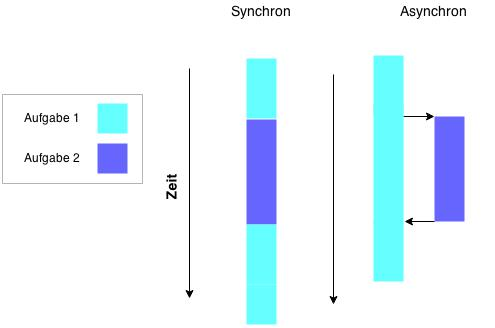
\includegraphics[width=8cm]{images/synchron_vs_asynchron.jpg}
  \caption{
    Synchron vs. Asynchron
  }
  \label{figure:syncron_vs_async_}
\end{figure}

Abbildung \ref{figure:syncron_vs_async_} zeigt den Unterschied zwischen synchron und asynchron. 

\subsection{Blocking vs Non-Blocking}

Unter einer blockierenden Prozedur versteht man eine Prozedur, welche den Aufrufer so lange blockiert bis diese abgeschlossen ist. Generell besitzt jeder Aufruf einer Prozedur in einem linearen Programmfluss einen blockierenden Charakter. Der Aufrufer einer Funktion wartet so lange bis die Funktion wieder zum Aufrufer zurückkehrt. 

Unter einer nicht blockierenden (eng. non-blocking) Prozedur versteht man eine Prozedur, die nicht auf den Abschluss einer Operation wartet, sondern sofort zum Aufrufer zurückspringt. Dabei werden mehrere Aufgaben gleichzeitig behandelt.  

In vielen Fällen wird eine blockierende Funktion im Zusammenhang mit I/O Operation gebracht, da diese Operationen nicht an die CPU eines Prozesses gebunden sind. Angenommen eine Prozedur soll eine Datei von der Festplatte einlesen. Die Prozedur fordert dazu das Betriebssystem auf die Datei einzulesen. Dabei kann die Datei entweder blockierend oder nicht blockierend eingelesen werden. Wird die blockierende Variante gewählt, so wird die Prozedur so lange pausiert bis die Datei vollständig eingelesen wurde. Wird die nicht blockierende Variante gewählt, so fordert die Prozedur das Betriebssystem auf die Datei zu lesen. Während das Betriebssystem die Datei noch einliest, wird die Prozedur fortgesetzt. Bei nicht blockierenden Prozeduren ist die aufrufende Prozedur selbst für die Synchronisation der Daten verantwortlich \cite[p. 47]{Erb2012}.

\begin{figure}[!htb]
  \centering
  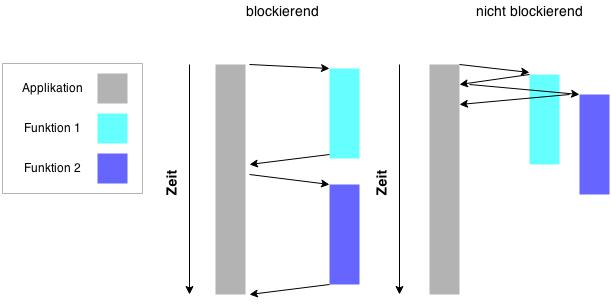
\includegraphics[width=9cm]{images/blocking_vs_nonblocking.jpg}
  \caption{
    Blocking vs Non-Blocking
  }
  \label{figure:blocking_vs_non_blocking}
\end{figure}

Abbildung \ref{figure:blocking_vs_non_blocking} zeigt die Unterschiede zwischen blockierenden und nicht blockierenden Prozeduren.

\subsection{Kombinationen}
Bei blockierenden oder nicht blockierenden Prozeduren geht es um die Art und Weise wie eine Prozedur auf dem Rechner ausgeführt wird. Bei synchronen oder asynchronen Prozeduren geht es um den Programmfluss. Kombiniert man die vorher genannten Konzepte so ergeben sich daraus vier unterschiedliche Kombinationen \cite[p. 48]{Erb2012}. Abbildung \ref{figure:synchron_blocking} zeigt alle vier Kombinationen auf einer Zeitachse. 

\begin{figure}[!htb]
  \centering
  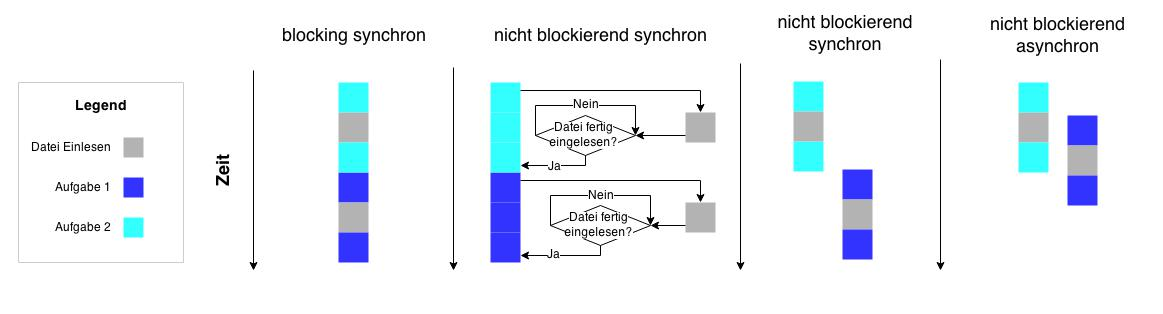
\includegraphics[width=16cm]{images/synchron_blocking.jpg}
  \caption{
    Unterschiedliche Kombinationen im Überblick
  }
  \label{figure:synchron_blocking}
\end{figure}

\subsubsection{Das blockierende und synchrone Modell}
Im blockierenden und synchronen Modell werden einzelne Operationen sequentiell abgearbeitet. Wird in diesem Modell eine blockierende Operation ausgeführt, wird die Prozedur so lange pausiert bis die blockierende Prozedur abgeschlossen ist. Danach wird der Programmfluss weiter ausgeführt bis die nächste blockierende Operation auftritt oder das Programm terminiert.

Ruft ein Prozess eine blockierende I/O Operation auf, so wird der Prozess so lange pausiert bis das Betriebssystem die Daten vollständig gelesen hat. Durch das blockierende und synchrone Modell wird die CPU nicht optimal ausgelastet. Da blockierende I/O Operationen den Prozess pausieren. In vielen Applikationen spielen I/O Operationen nur eine nebensächliche Rolle. Für Applikationen, welche viele I/O Operationen benötigen, ist dieses Modell nur bedingt geeignet \cite[p. 48]{Erb2012}.


\subsubsection{Das nicht blockierende synchrone Modell}

Bei diesem Modell kehrt eine Prozedur sofort nach dem Aufruf zum Aufrufer zurück. Das Resultat der aufgerufenen Prozedur könnte in diesem Fall noch nicht verfügbar sein. Der Aufrufer selbst muss sich um die Synchronisierung der Daten zwischen den beiden Prozeduren kümmern. Dabei muss der Aufrufer selbst den Programmfluss unterbrechen bis die Prozedur abgeschlossen ist. 

Das nicht blockierende synchrone Modell führt zu unnötigem Ressourcenverbrauch, da die Applikation zwar prinzipiell nicht blockiert, jedoch trotzdem wartet bis eine Operation zu Ende ist. Ein möglicher Ablauf einer Implementierung ist in Abbildung \ref{figure:synchron_blocking} (zweite Abbildung) zu sehen. Es wird eine Schleife verwendet, die bei jedem Durchgang fragt, ob die I/O Operation bereits abgeschlossen ist \cite[p. 48]{Erb2012}.

\subsubsection{Das blockierende asynchrone Modell}

Das blockierende asynchrone Modell verwendet einen zweiten Programmfluss für die Applikation. Durch den blockierenden Charakter verhält sich das blockierende asynchrone Modell ähnlich dem blockierenden synchronen Model. 

\subsubsection{Das nicht blockierende asynchrone Modell}
Beim nicht blockierenden asynchronen Modell kehrt eine blockierende Operation sofort an die aufrufende Funktion zurück. Die aufrufende Funktion kann in der Zeit des blockierenden Aufrufes andere Aufgaben erledigen. Durch das nicht blockierende asynchrone Modell wird die I/O Operation direkt im Kernel des Betriebssystems abgearbeitet. Ist die Operation abgeschlossen, wird entweder ein Ereignis ausgelöst oder eine Callback Funktion ausgeführt \cite[p. 48]{Erb2012}.

Ein Grund warum das asynchrone nicht blockierende Modell schneller sein kann als die beiden synchronen Modelle sind I/O Operationen, die den Prozess blockieren\ref{subsection: io_operationen}. Angenommen eine Applikation möchte zwei Aufgaben erledigen bei der die erste Aufgabe eine Datei vom Dateisystem einliest. Im Falle der beiden synchronen Modelle müsste die Aufgabe 1 auf das fertige Einlesen der Datei warten. Dies kann entweder auf Kernelebene funktionieren (= synchrones blockierendes Modell) oder auf Applikationsebene (= synchrones nicht blockierendes Modell) passieren \cite[]{Pet2015}. 

Im asynchronen nicht blockierenden Modell kann die Applikation die Aufgabe 1 ausführen bis die Operation blockiert. Während der Kernel die Datei einliest kann die Applikation die Aufgabe 2 ausführen und nach dem Terminieren der Aufgabe 2 wird die Aufgabe 1 abgeschlossen. Dadurch macht das Programm immer einen Fortschritt, ohne dass es auf auf Daten vom Kernel warten muss \cite[]{Pet2015}.


\subsection{Zusammenfassung}

In diesem Kapitel wurden die Grundlagen für asynchrone Programmierung besprochen. Dabei kann man Programme grundsätzlich in vier unterschiedliche Kategorien einteilen:

\begin{itemize}
  \item blockierend und synchron
  \item nicht blockierend und synchron
  \item blockierend und asynchron
  \item nicht blockierend und asynchron
\end{itemize}

Viele Anwendungen, welche nur wenige I/O Operationen besitzen, verwenden das blockierende und synchrone Modell, da es einen linearen Programmfluss erlaubt. Das nicht blockierende und synchrone Modell verlagert das Warten auf I/O Operationen vom Betriebssystem in die Applikation, was zu einem unnötigen Ressourcenverbrauch führen kann. Das asynchrone und nicht blockierende Modell bietet die Möglichkeit die CPU bestmöglich auszunutzen da die Applikation während der I/O Operation eine andere Aufgabe ausführen kann.